\documentclass[10pt, compress]{beamer}

\usetheme{m}

\usepackage{booktabs,pgf-pie}
\usepackage[scale=2]{ccicons}
\graphicspath{{./images/}}

\usepgfplotslibrary{dateplot}


\title{JBomberman}
\subtitle{}
\date{28.05.2015}
\author{Silvan Adrian, Fabian Binna, Pascal Kistler}
\institute{Hochschule für Technik Rapperswil \newline \newline
Webseite: \textcolor{red}{\href{http://se2p.zonk.io}{http://se2p.zonk.io}}}

\begin{document}

\maketitle

%Ablauf
\begin{frame}{fragile}
	\frametitle{Ablauf}
	\begin{itemize}
	\item Idee
	\item Architektur
	\item Risiko
	\item Demonstration
	\item Probleme und Lösungen
	\item Statistiken
	\item Usability Test
	\item Fazit
	\item Fragen
	\end{itemize}
\end{frame}


\section{Idee}
%Idee
\begin{frame}[fragile]
  \frametitle{Idee}
	\begin{itemize}
	  \item Projekt das Spass macht und fordert
	  \item Netzwerkbasierend
	  \item Klon eines Spiel
	  \item Erste Erfahrungen in der Spielentwicklung
	  \item Eigene Engine
	\end{itemize}
\end{frame}



\section{Anforderungen  Konzepte}

%Anforderungen
\begin{frame}[fragile]
	\frametitle{Anforderungen}
	Bombermanklon: Mehrspielermodus mit 2-4 Spieler
	\begin{center}
	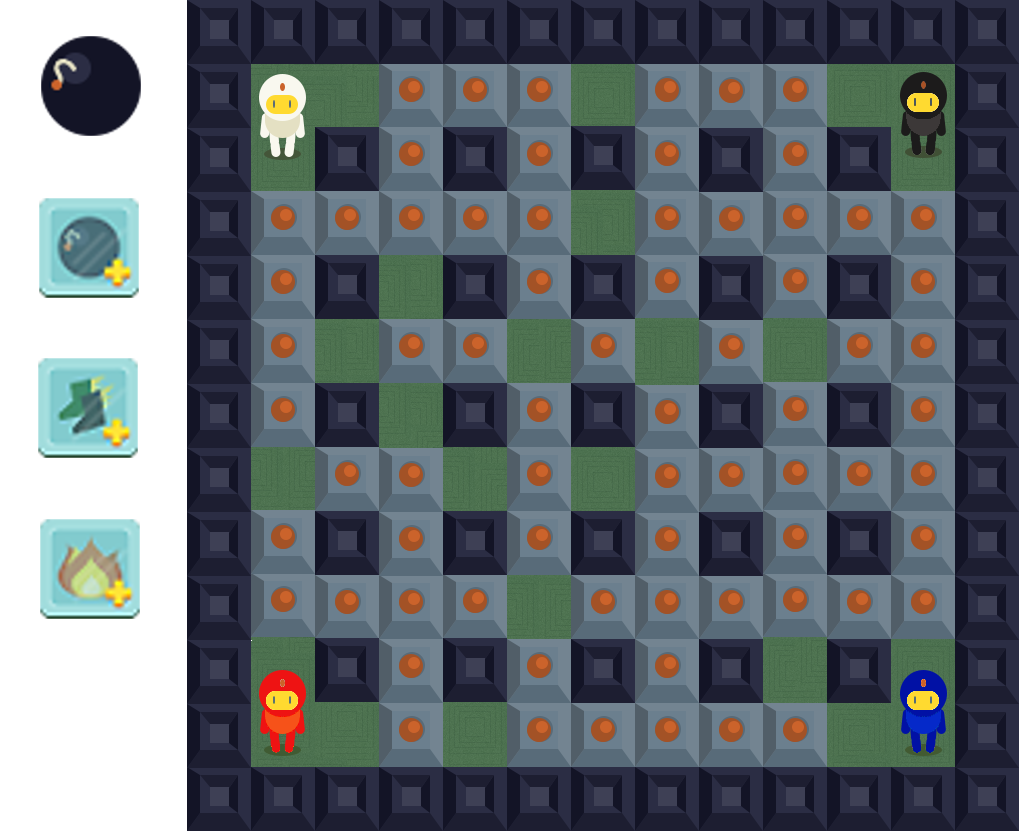
\includegraphics[scale=0.8]{bombermangame}
	\end{center}
\end{frame}

%Domain Modell
\begin{frame}[fragile]
  \frametitle{Domain Modell}
	\begin{center}
	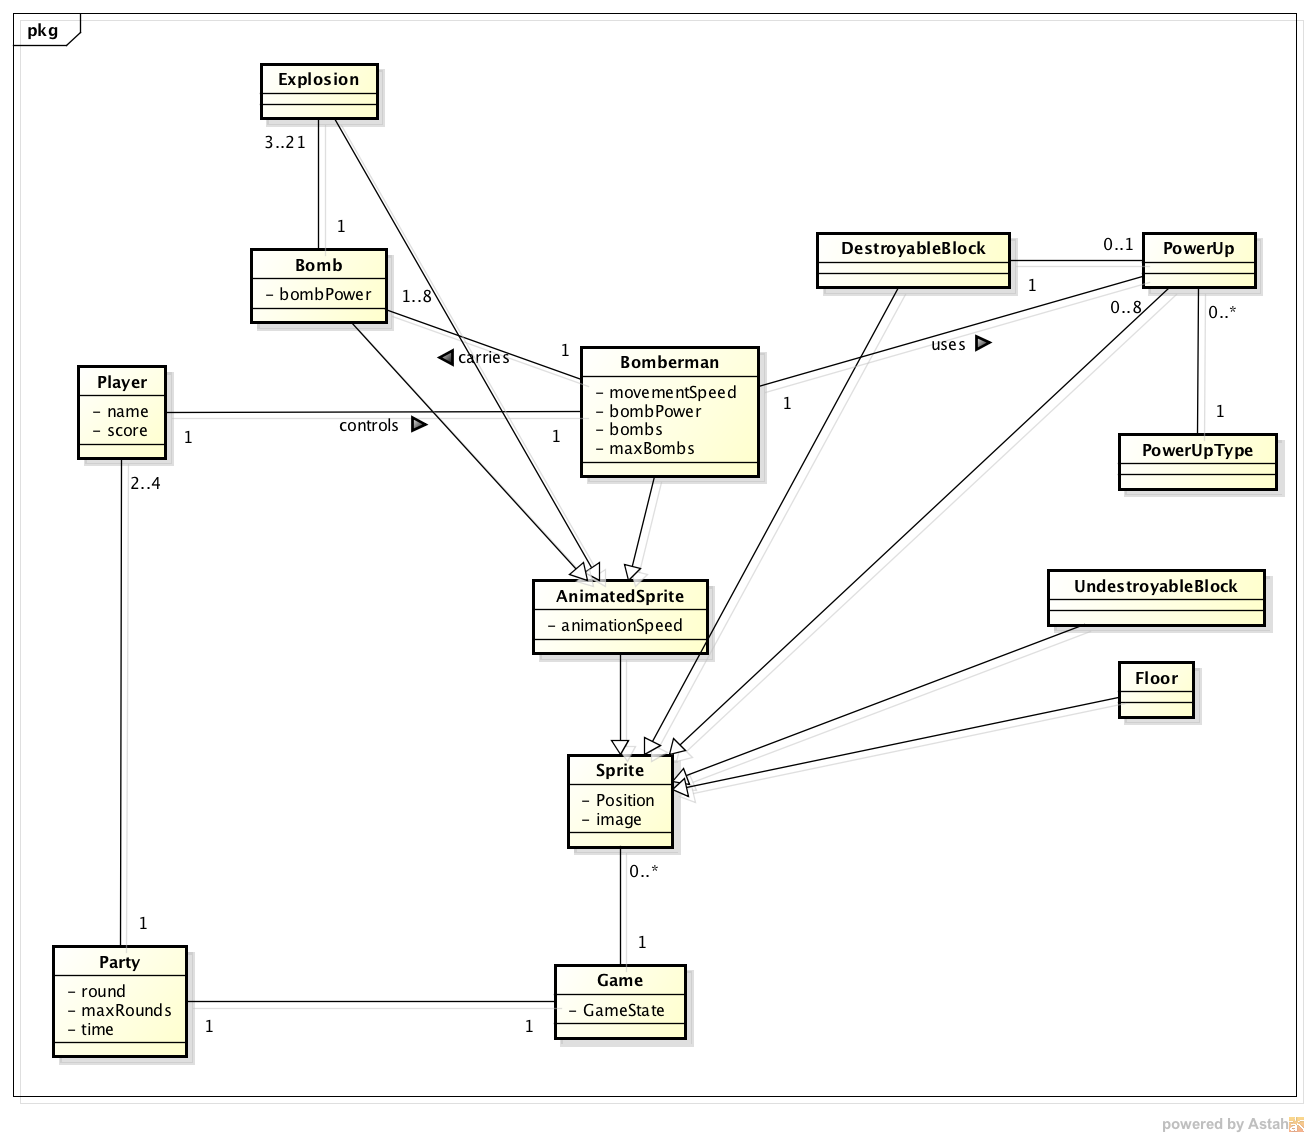
\includegraphics[scale=0.25]{Strukturdiagramm_JBomberman}
	\end{center}
\end{frame}

%Design
\begin{frame}{fragile}
  \frametitle{Architektur: Logische Sicht}
	\begin{center}
	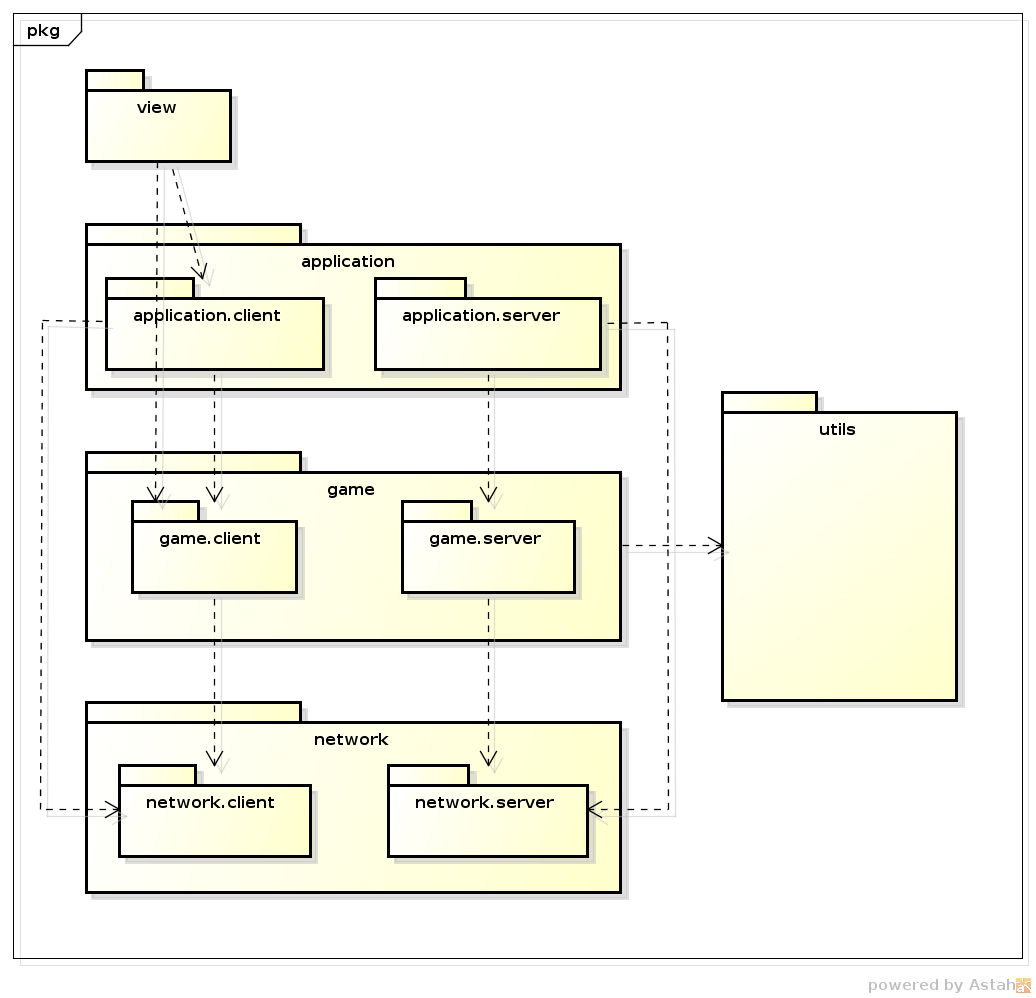
\includegraphics[scale=0.3]{LogischeSicht}
	\end{center}
\end{frame}

\begin{frame}{fragile}
	\frametitle{Architektur: Server}
	\begin{center}
	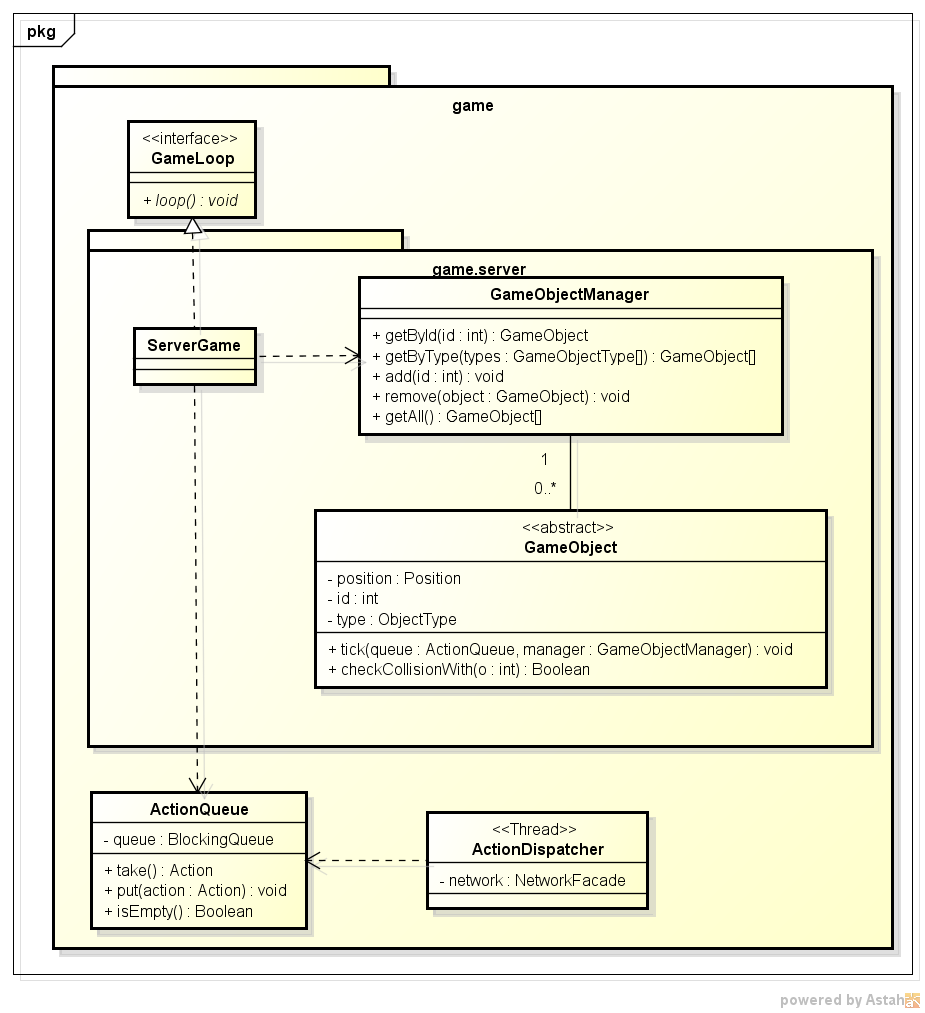
\includegraphics[scale=0.3]{ClassDiagramGameServer}
	\end{center}
\end{frame}

\begin{frame}{fragile}
	\frametitle{Architektur: Client}
	\begin{center}
	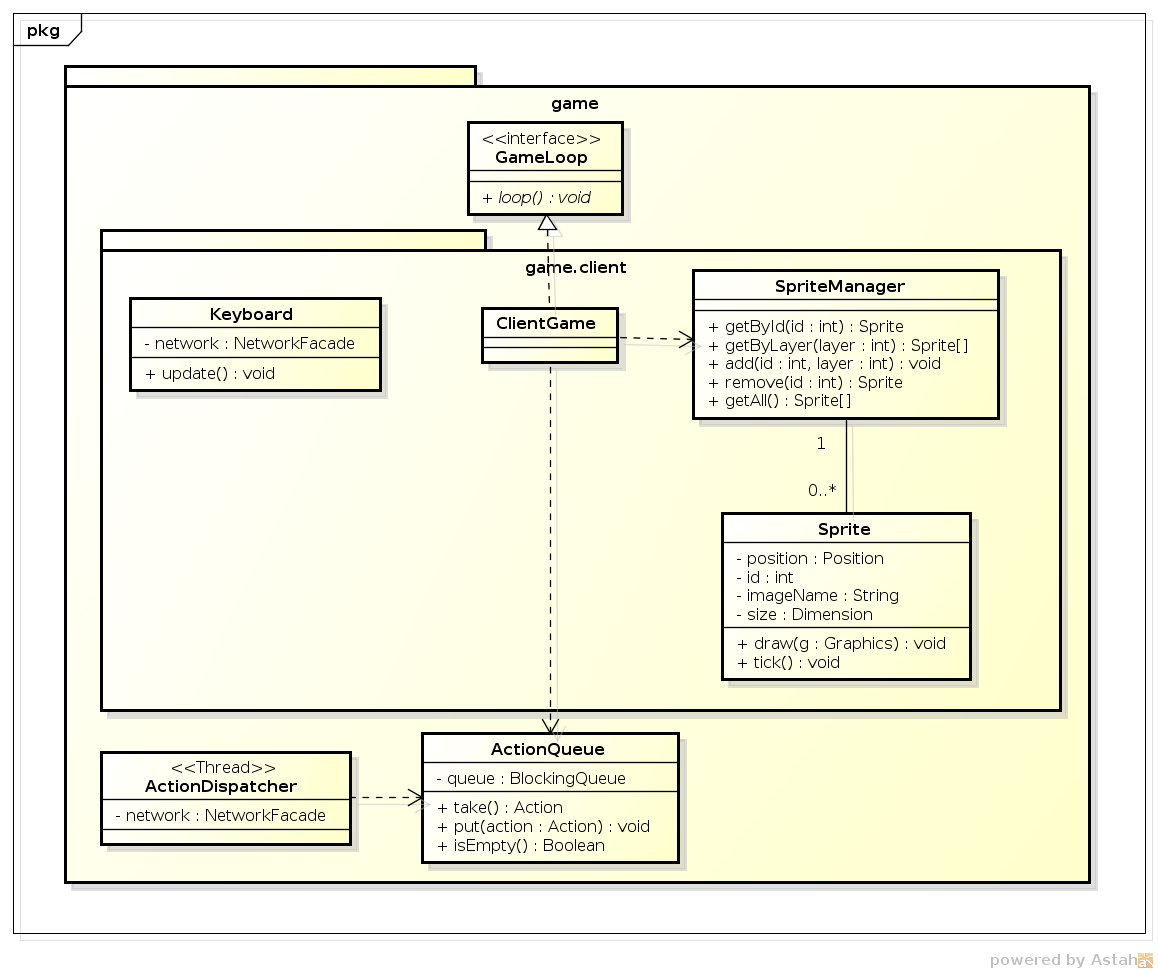
\includegraphics[scale=0.3]{ClassDiagramGameClient}
	\end{center}
\end{frame}

%Externes Design
\begin{frame}{fragile}
	\frametitle{Externes Design: Client}
	\begin{center}
	  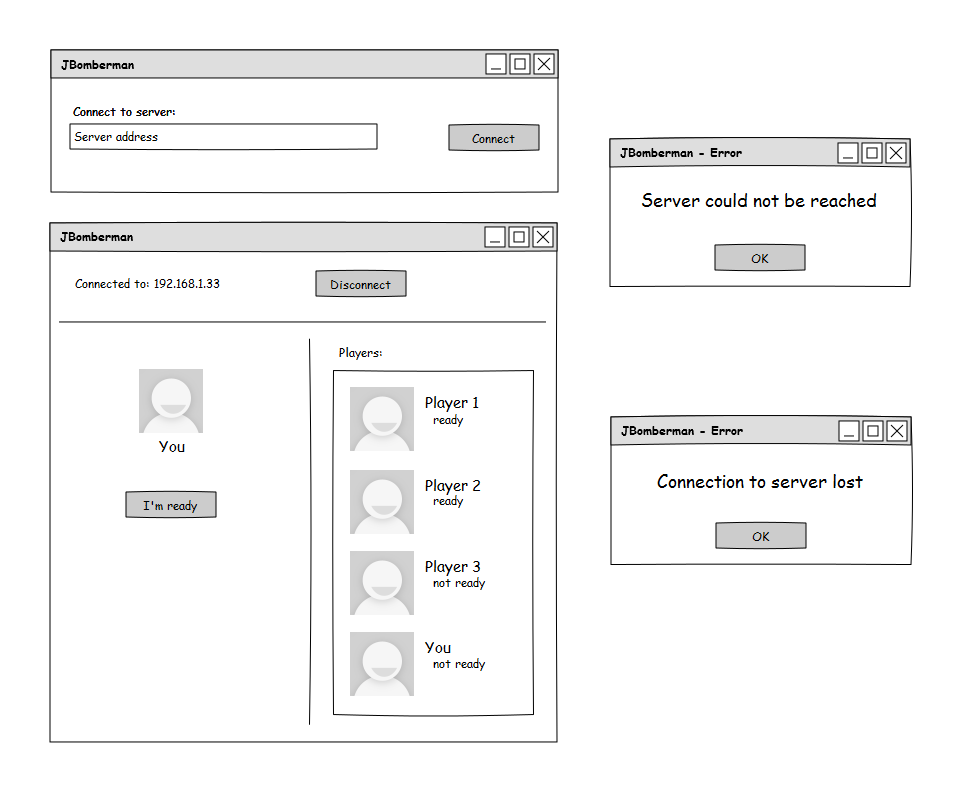
\includegraphics[scale=0.25]{client}
	\end{center}
	
\end{frame}

\begin{frame}{fragile}
	\frametitle{Externes Design: Game}
	\begin{center}
	  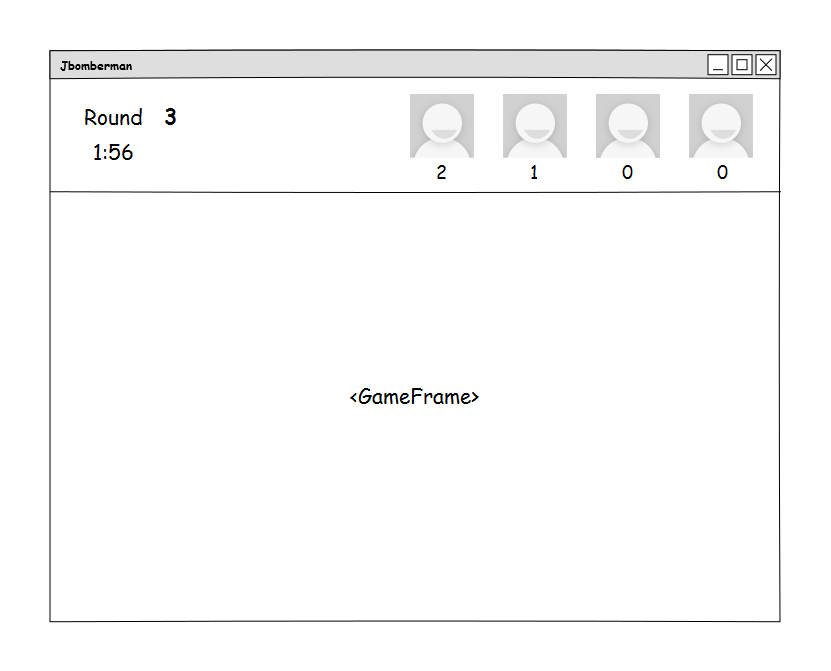
\includegraphics[scale=0.3]{game}
	\end{center}
	
\end{frame}

\begin{frame}{fragile}
	\frametitle{Externes Design: Server}
	\begin{center}
	  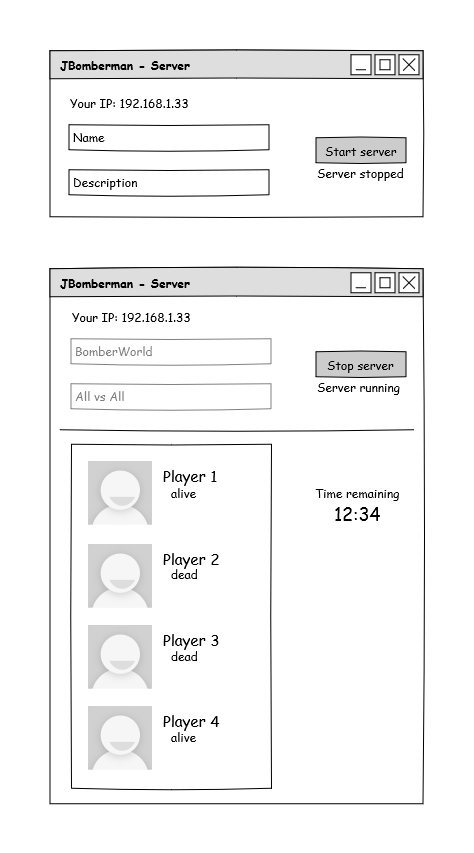
\includegraphics[scale=0.25]{server}
	\end{center}
	
\end{frame}

%High Risks Tasks
\begin{frame}{fragile}
	\frametitle{Risiken}
	\begin{itemize}
	\item Netzwerkperformance
	\item Performance der Applikation
	\item Komplexität Architektur/Code
	\end{itemize}
\end{frame}

%Demo
\plain{Demonstration}

%probleme & Lösungen
\begin{frame}{fragile}
	\frametitle{Probleme}
	\begin{itemize}
		\item RabbitMQ
		\item Threads
		\item Git
		\item VPN Bug
	\end{itemize}
\end{frame}

\begin{frame}{fragile}
  \frametitle{STAN}
  \begin{center}
    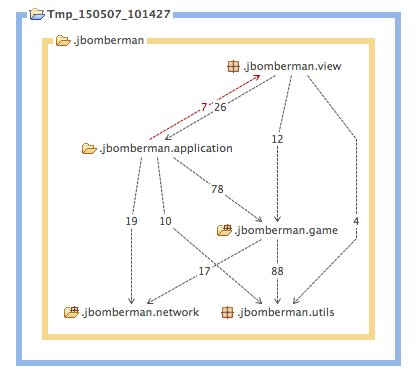
\includegraphics[scale=0.4]{stan}
  \end{center}
    
\end{frame}


%Statistiken
\section{Statistiken}
\begin{frame}{fragile}
  \frametitle{Iterationen}
      \begin{tikzpicture}
      \begin{axis}[
        mbarplot,
        xlabel={Iteration},
        ylabel={Stunden},
        width=\textwidth,
        height=6cm,
        symbolic x coords={Inception,Elaboration1,Elaboration2,Elaboration3,
        Construction1, Construction2, Construction3, Transition},
        x tick label style={rotate=45,anchor=east},
      ]

      \addplot plot coordinates {
      (Inception, 5.00)
       (Elaboration1, 50.00) 
      (Elaboration2, 54.00) 
      (Elaboration3, 77.00)
      (Construction1, 35.00) 
      (Construction2, 50.50)
      (Construction3, 67.25) 
      (Transition, 27.00)
       };
      \addplot plot coordinates {
      (Inception, 4.50) 
      (Elaboration1, 66) 
      (Elaboration2, 52.00) 
      (Elaboration3, 89.25)
      (Construction1, 44.00) 
      (Construction2, 49.50)
      (Construction3, 63.25 ) 
      (Transition, 16.25)
      };

      \legend{Soll, Ist}

      \end{axis}
       \end{tikzpicture}
     \end{frame}
     
\begin{frame}{fragile}
   \frametitle{Wochen}
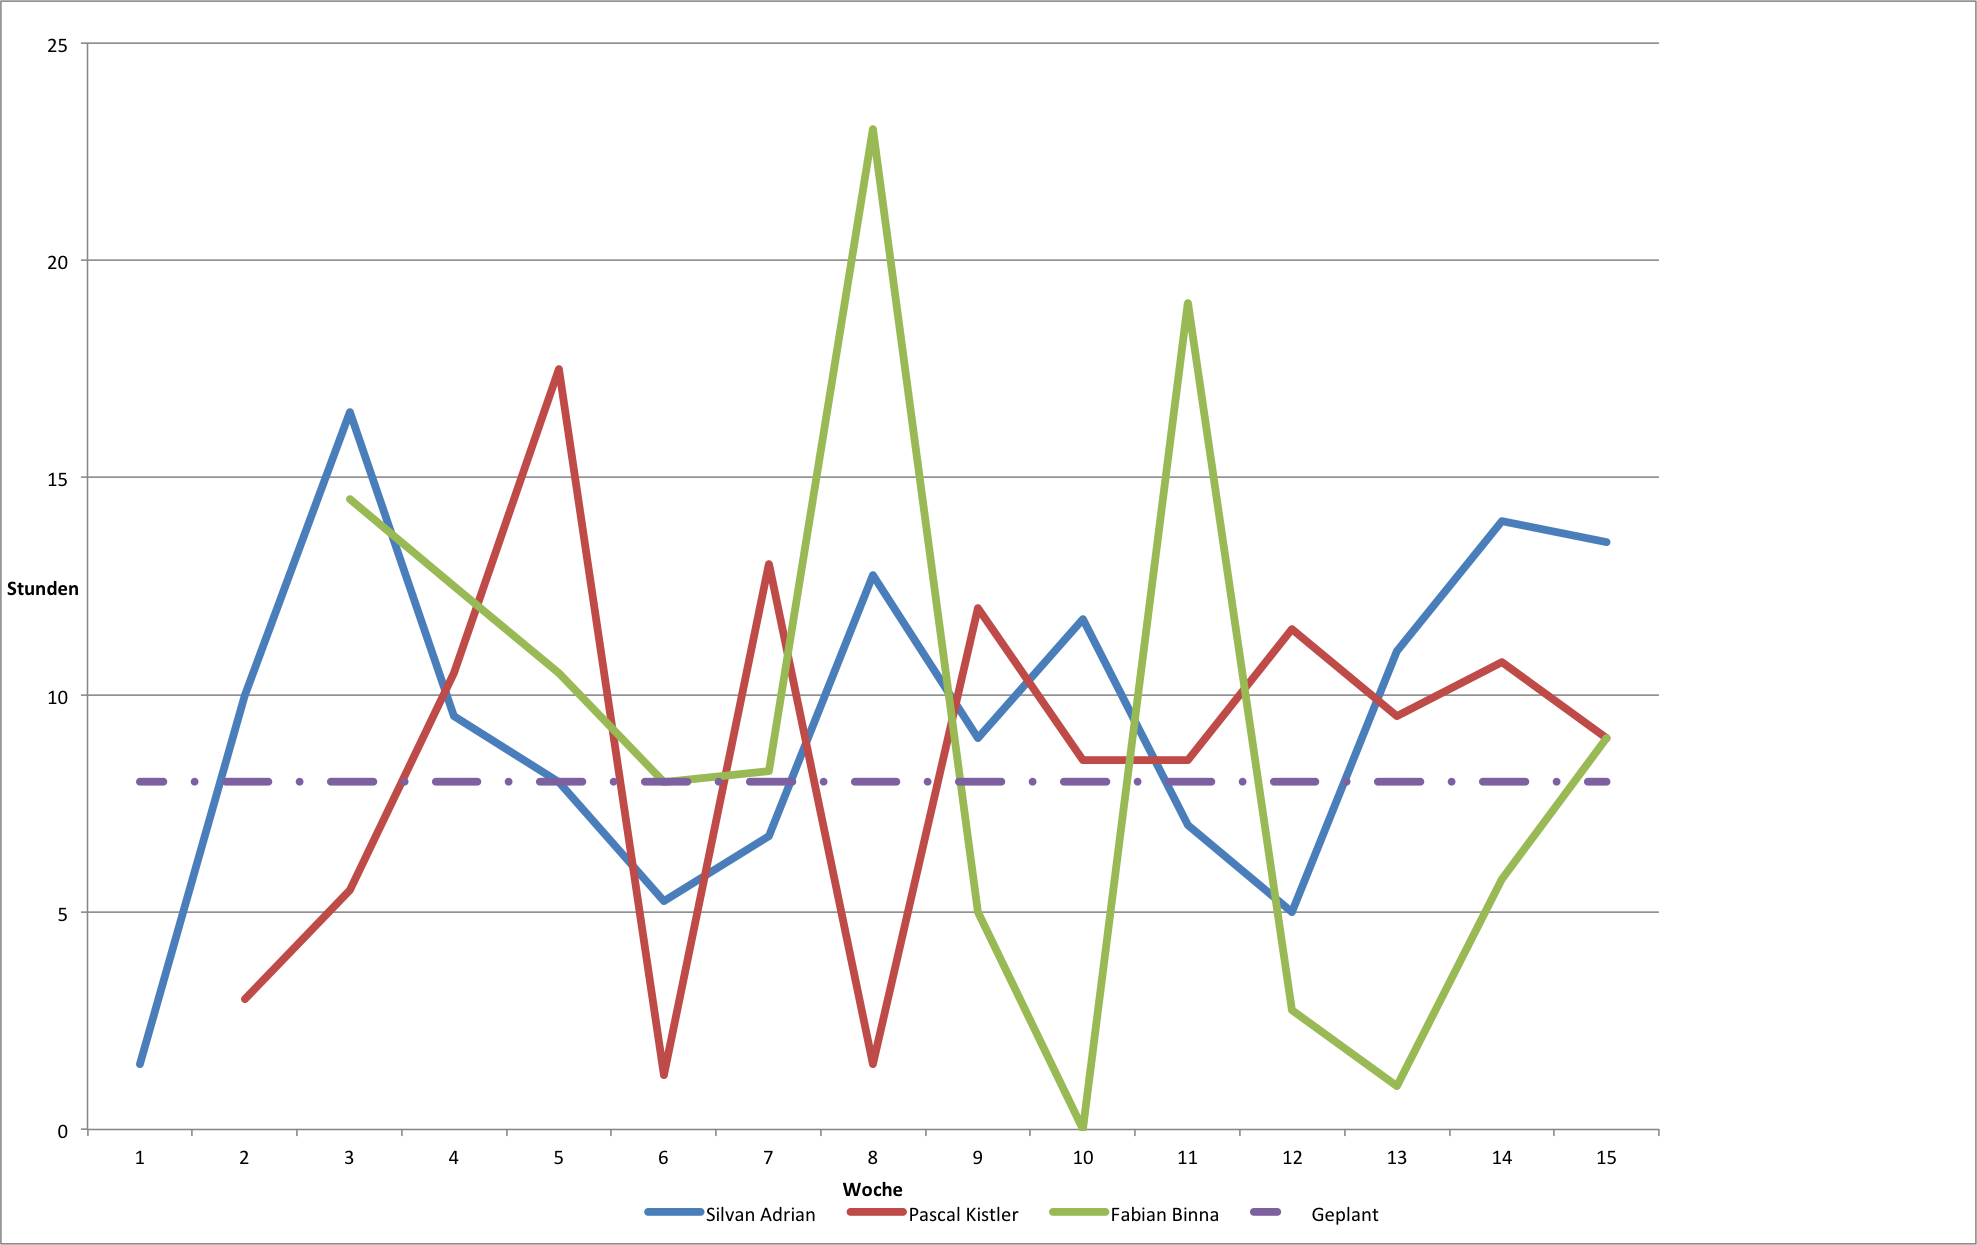
\includegraphics[scale=0.35]{wochenstunden}
\end{frame} 
    
\begin{frame}{fragile}
   \frametitle{Personen}
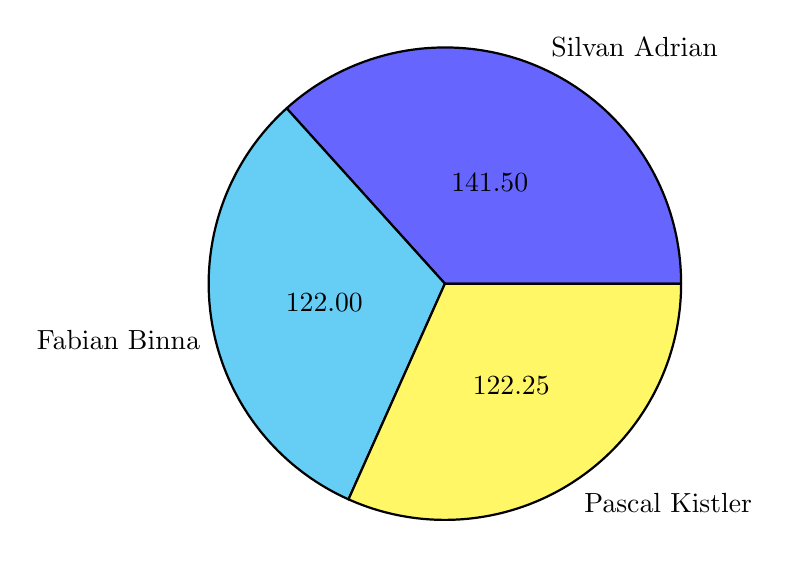
\begin{tikzpicture}
\pie[sum=385.75]{141.50/Silvan Adrian, 122.00/Fabian Binna, 122.25/Pascal Kistler}
\end{tikzpicture}
\end{frame}

\begin{frame}{fragile}
   \frametitle{Kategorien}
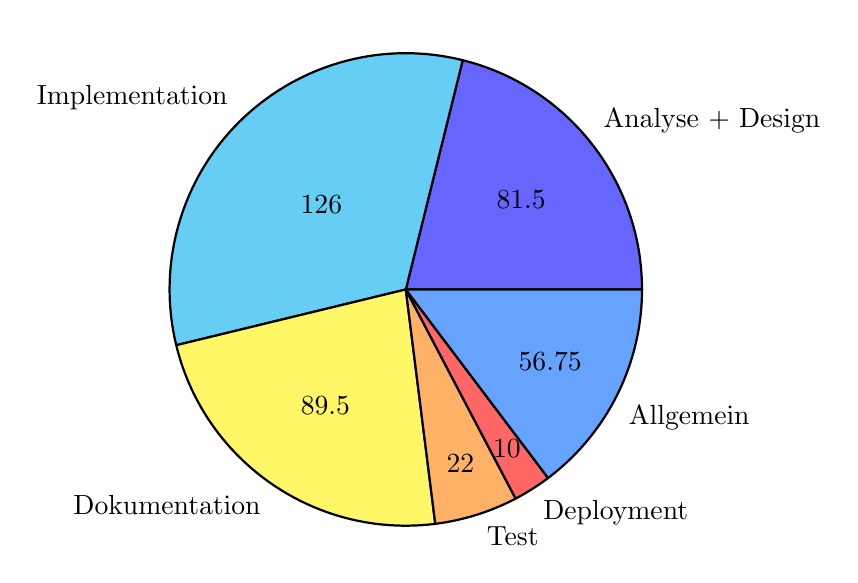
\begin{tikzpicture}
\pie[sum=385.75]{81.5/Analyse + Design,126/Implementation,89.5/Dokumentation,22/Test,10/Deployment ,56.75/Allgemein}
\end{tikzpicture}
\end{frame}

\begin{frame}{fragile}
   \frametitle{Code Statistik}
  \begin{columns}[onlytextwidth]
    \column{0.5\textwidth}
\begin{itemize}
  \item Anzahl Klassen: 59
  \item Code Zeilen: 3266
  \item Ca.: 55 Zeilen/Klasse
\end{itemize}
\column{0.5\textwidth}
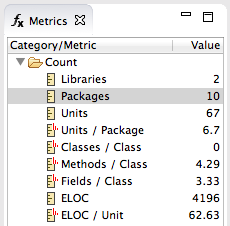
\includegraphics[width=\textwidth]{stan-metrics}
\end{columns}

\end{frame}
%Findbugs
\begin{frame}{fragile}
   \frametitle{Findbugs}
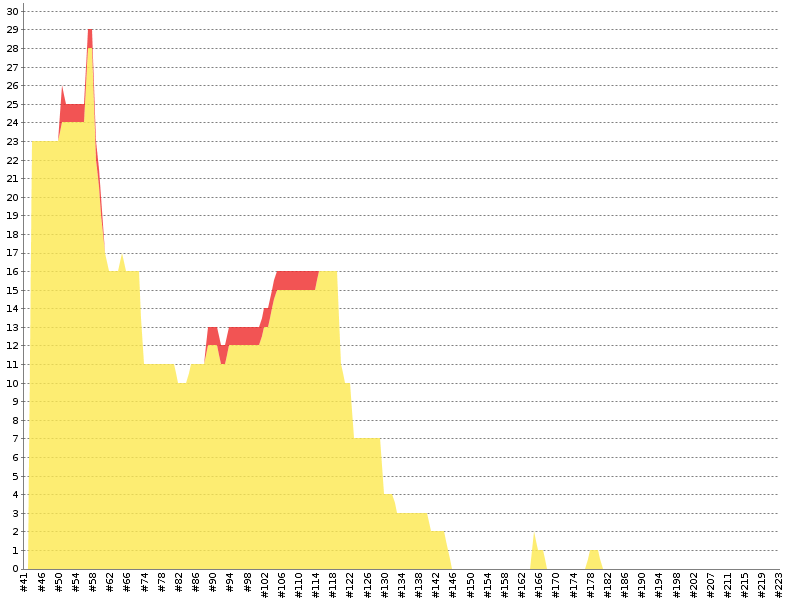
\includegraphics[scale=0.35]{findbugs}
\end{frame}

%Git
\begin{frame}{fragile}
   \frametitle{GIT}
   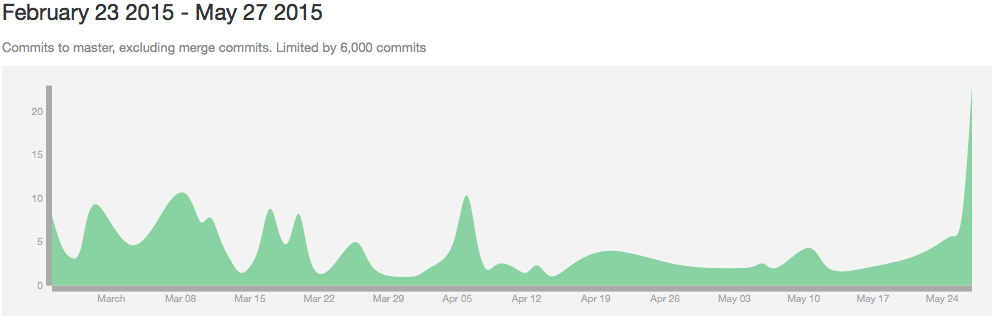
\includegraphics[scale=0.3]{doku}\newline
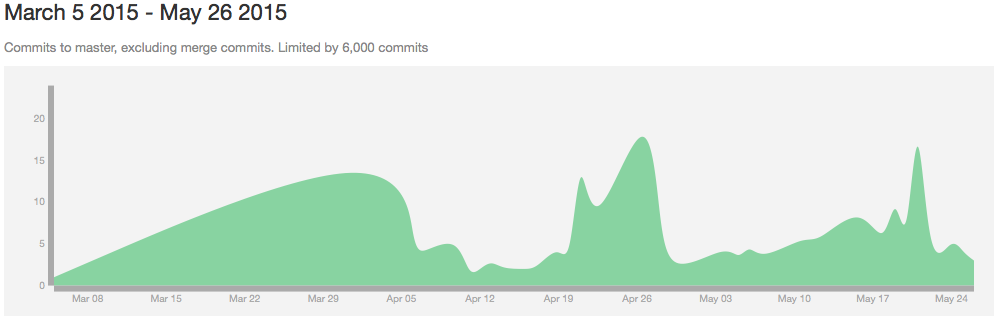
\includegraphics[scale=0.3]{code}
\end{frame}


%Usability Test
\begin{frame}{fragile}
  \frametitle{Usability Test}
  \begin{columns}[onlytextwidth]
    \column{0.5\textwidth}
  \begin{itemize}
    \item 2 Tests (RC1 und RC2)
    \item Jeweils 1 und 2 Teilnehmer
    \item Fragebogen nach Quensbery (5 E's)
    \item Sehr gute Unterstützung fürs Bugs finden
  \end{itemize}
  
  \column{0.5\textwidth}
  \begin{center}
    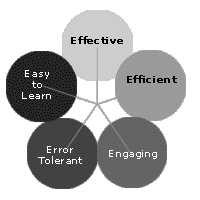
\includegraphics[width=0.8\textwidth]{quesenbery}
  \end{center}
   
  \end{columns}
\end{frame}

%Fazit,Lessons learned
\section{Fazit}
\begin{frame}{Summary}
\frametitle{Fazit}
\begin{columns}[onlytextwidth]
    \column{0.5\textwidth}
      \textbf{Positives}
\begin{itemize}
  \item Teamarbeit
  \item Neue Technologien gelernt
  \item Neue Tools verwendet und kennengelernt
\end{itemize}

    \column{0.5\textwidth}
    \textbf{Negatives}
\begin{itemize}
  \item Projektmanagement
  \item Viel genauer Anforderungen beschreiben/setzen
  \item Dokumentation
\end{itemize}
  \end{columns}

\end{frame}

\plain{Fragen?}

\end{document}
